\scanpage{23}
\uline{Lemme} 1 Soit $f:S'\longrightarrow S$ un épimorphisme propre de schémas [\inserted{loc} noethériens], et \deleted{$\unsure{Z}$} $X$ un schéma \inserted{formellement} non ramifié sur $S$. Alors la suite
\margin{\figure{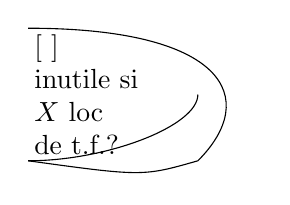
\begin{tikzpicture}\node[align=left,text width=2cm,inner sep=2pt](m){[\ ]\\inutile si\\$X$ \uline{loc}\\de t.f.?};\draw (m.north west) .. controls +(2.5,0) and +(.8,.8) .. (m.south east);\draw (m.south east) .. controls +(-.7,-.2) .. (m.south west);\draw (m.east) .. controls +(0,-.4) and +(1,0) .. (m.south west);\end{tikzpicture}}}
\diagram{\begin{tikzcd}[ampersand replacement=\&,column sep=large]\operatorname{Hom}_S(S,X)\arrow[r]\&\operatorname{Hom}_S(S',X)\arrow[r,shift left=.5ex]\arrow[r,dash,shift right=.5ex]\&\operatorname{Hom}_S(S'',X)\end{tikzcd}}
est exacte, où $S''=S'\times_S S'$.

\unsure{NB} le fait que $f$ est un épimorphisme s'exprime par la condition que l'hom
\[
\underline O_S\longrightarrow f_*(O_{S'})
\]
est \uline{injectif}.

Soit $g':S'\longrightarrow X$ tel que $g'\operatorname{pr}_1=g'\operatorname{pr}_2$, à montrer que $g'$ se factorise par $S$. Tout d'abord il se factorise par $S$ en \unsure{prenant} une application continue, soit $g_0$, et
\[
f^{-1}(g_0^{-1}(\underline O_X))\simeq g'^{-1}(O_X)\longrightarrow O_{S'}
\]
adjoint un hom
\[
g_0^{-1}(O_X)\longrightarrow f_*(O_{S'});
\]
\diagram{\begin{tikzcd}[ampersand replacement=\&,column sep=small,row sep=small]\&\&X\arrow[d]\\S''\arrow[r,shift left=.5ex,"p_1"]\arrow[r,shift right=.5ex,"p_2"']\arrow[rr,bend right=30,"h"']\&S'\arrow[ur,"g'"]\arrow[r,"f"']\&S\arrow[u,dashed,bend right=20,"g_0"']\end{tikzcd}}
l'hyp. $g'\operatorname{pr}_1=g'\operatorname{pr}_2$ s'exprime par le fait que $g_0^{-1}(\underline O_X)$ s'envoie dans
\[
\mathcal A=\operatorname{Ker}(f_*(O_{S'})\rightrightarrows\deleted{\unsure{f_*}}h_*(\underline O_{S''}))
\]
donc $g'$ se factorise par
\[
S'\longrightarrow\operatorname{Spec}(\mathcal A)=S'_1\longrightarrow X.
\]
Or EGA III 3 implique évidemment que $S'_1\longrightarrow S'$ est \inserted{fini,} \uline{radiciel}, c'est d'ailleurs un épimorphisme car $\underline O_S\hookrightarrow\deleted{\unsure{f_*\underline O_S}}\mathcal A\hookrightarrow f_*(O_{S'})$, $f$ étant un épimorphisme. On est donc ramené à prouver le
\margin{\uline{lemme}}

\uline{Corollaire} 1 Soit $f:S'\mathbin{-}S$ un épimorphisme de schémas \deleted{\unsure{noethériens}}, $f$ \deleted{fini} \inserted{entier} radiciel, et $X$ \deleted{non ramifié} \inserted{\deleted{loc de t.f.}\unsure{formelt}} sur $S$; \deleted{\unsure{Alors $f$ fini}} \inserted{(on \unsure{suppose} $f$ fini et $S$ loc. noeth, ou $X\mathbin{-}S$ loc. de t.f.)} Alors
\[
\operatorname{Hom}_S(S,X)\mathbin{-}\operatorname{Hom}_S(S',X)\quad\text{est \uline{bijectif}}.
\]
\mspage{22}
